\subsection{Regulador L78XX}
La mayoría de los reguladores son circuitos integrados y tienen tres terminales:
una de entrada, una de salida y una de referencia (o ajuste). Primero se filtra
la entrada al regulador con un capacitor para reducir el rizo a $<10\%$.
Típicamente, los reguladores de voltaje proporcionan una salida constante con un
alto rechazo a los rizos.

Los reguladores de tres terminales diseñados para voltajes de salida fijos
requieren sólo capacitores externos para completar la parte de regulación de la
fuente de alimentación. El filtrado se realiza por un capacitor de gran valor
entre el voltaje de entrada y tierra. Un capacitor de salida está conectado de
la salida a tierra para mejorar la respuesta transitoria \cite{Floyd}.

En la \textbf{figura~\ref{circuito09}} se muestra un circuito regulador
\textbf{L7809CV} que fija el voltaje a $+9[\text{V}]$ filtrado por un capacitor
de $470[\mu\text{F}]$ en la entrada y un capacitor de $10[\mu\text{F}]$ para la
salida.

\begin{figure}[!h]
\centering
\includegraphics[scale=1.1]{diagramas/09.regulador1.eps}
\caption{Regulación de voltaje con \textbf{L7809CV}.}
\label{circuito09}
\end{figure}

\subsubsection{Simulación}
Se utilizó el software \emph{Quite Universal Circuit Simulator.} versión 23.3.1
para la simulación de la regulación de voltaje con el circuito integrado
\textbf{L7809CV} este puede verse en la \textbf{figura~\ref{simulacion09}}.

\begin{figure}[!h]
\centering
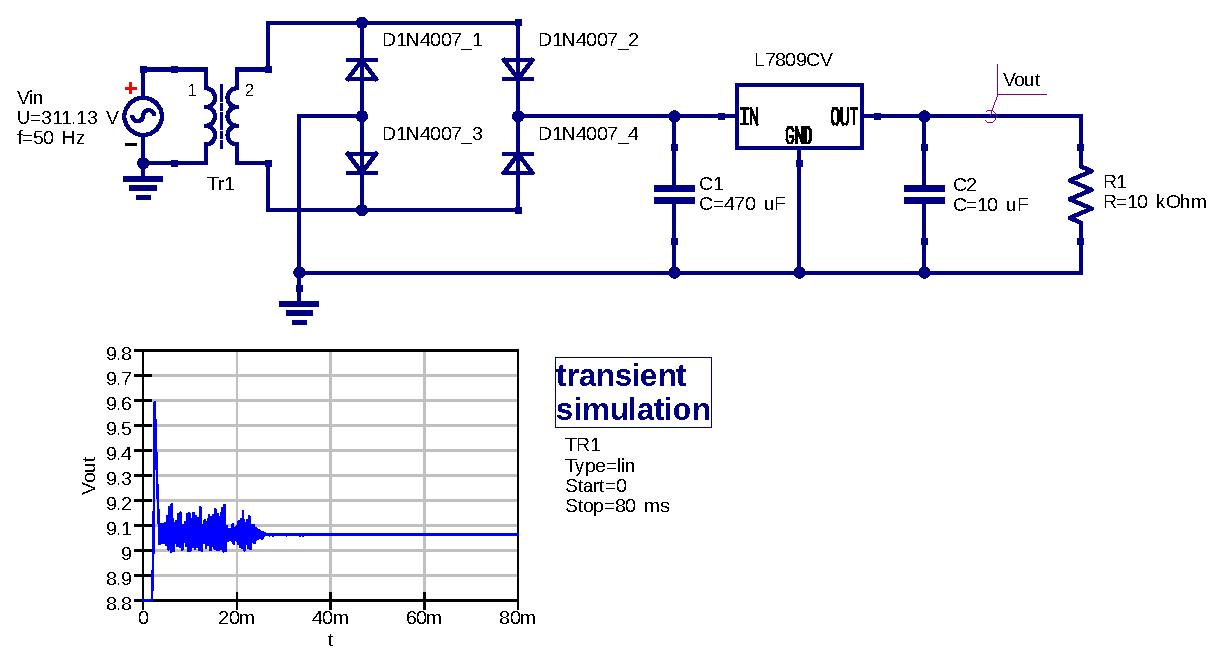
\includegraphics[scale=0.75]{simulacion/09.regulador1.eps}
\caption{Simulación del regulador \textbf{L7809CV}.}
\label{simulacion09}
\end{figure}

\begin{figure}[!h]
\centering
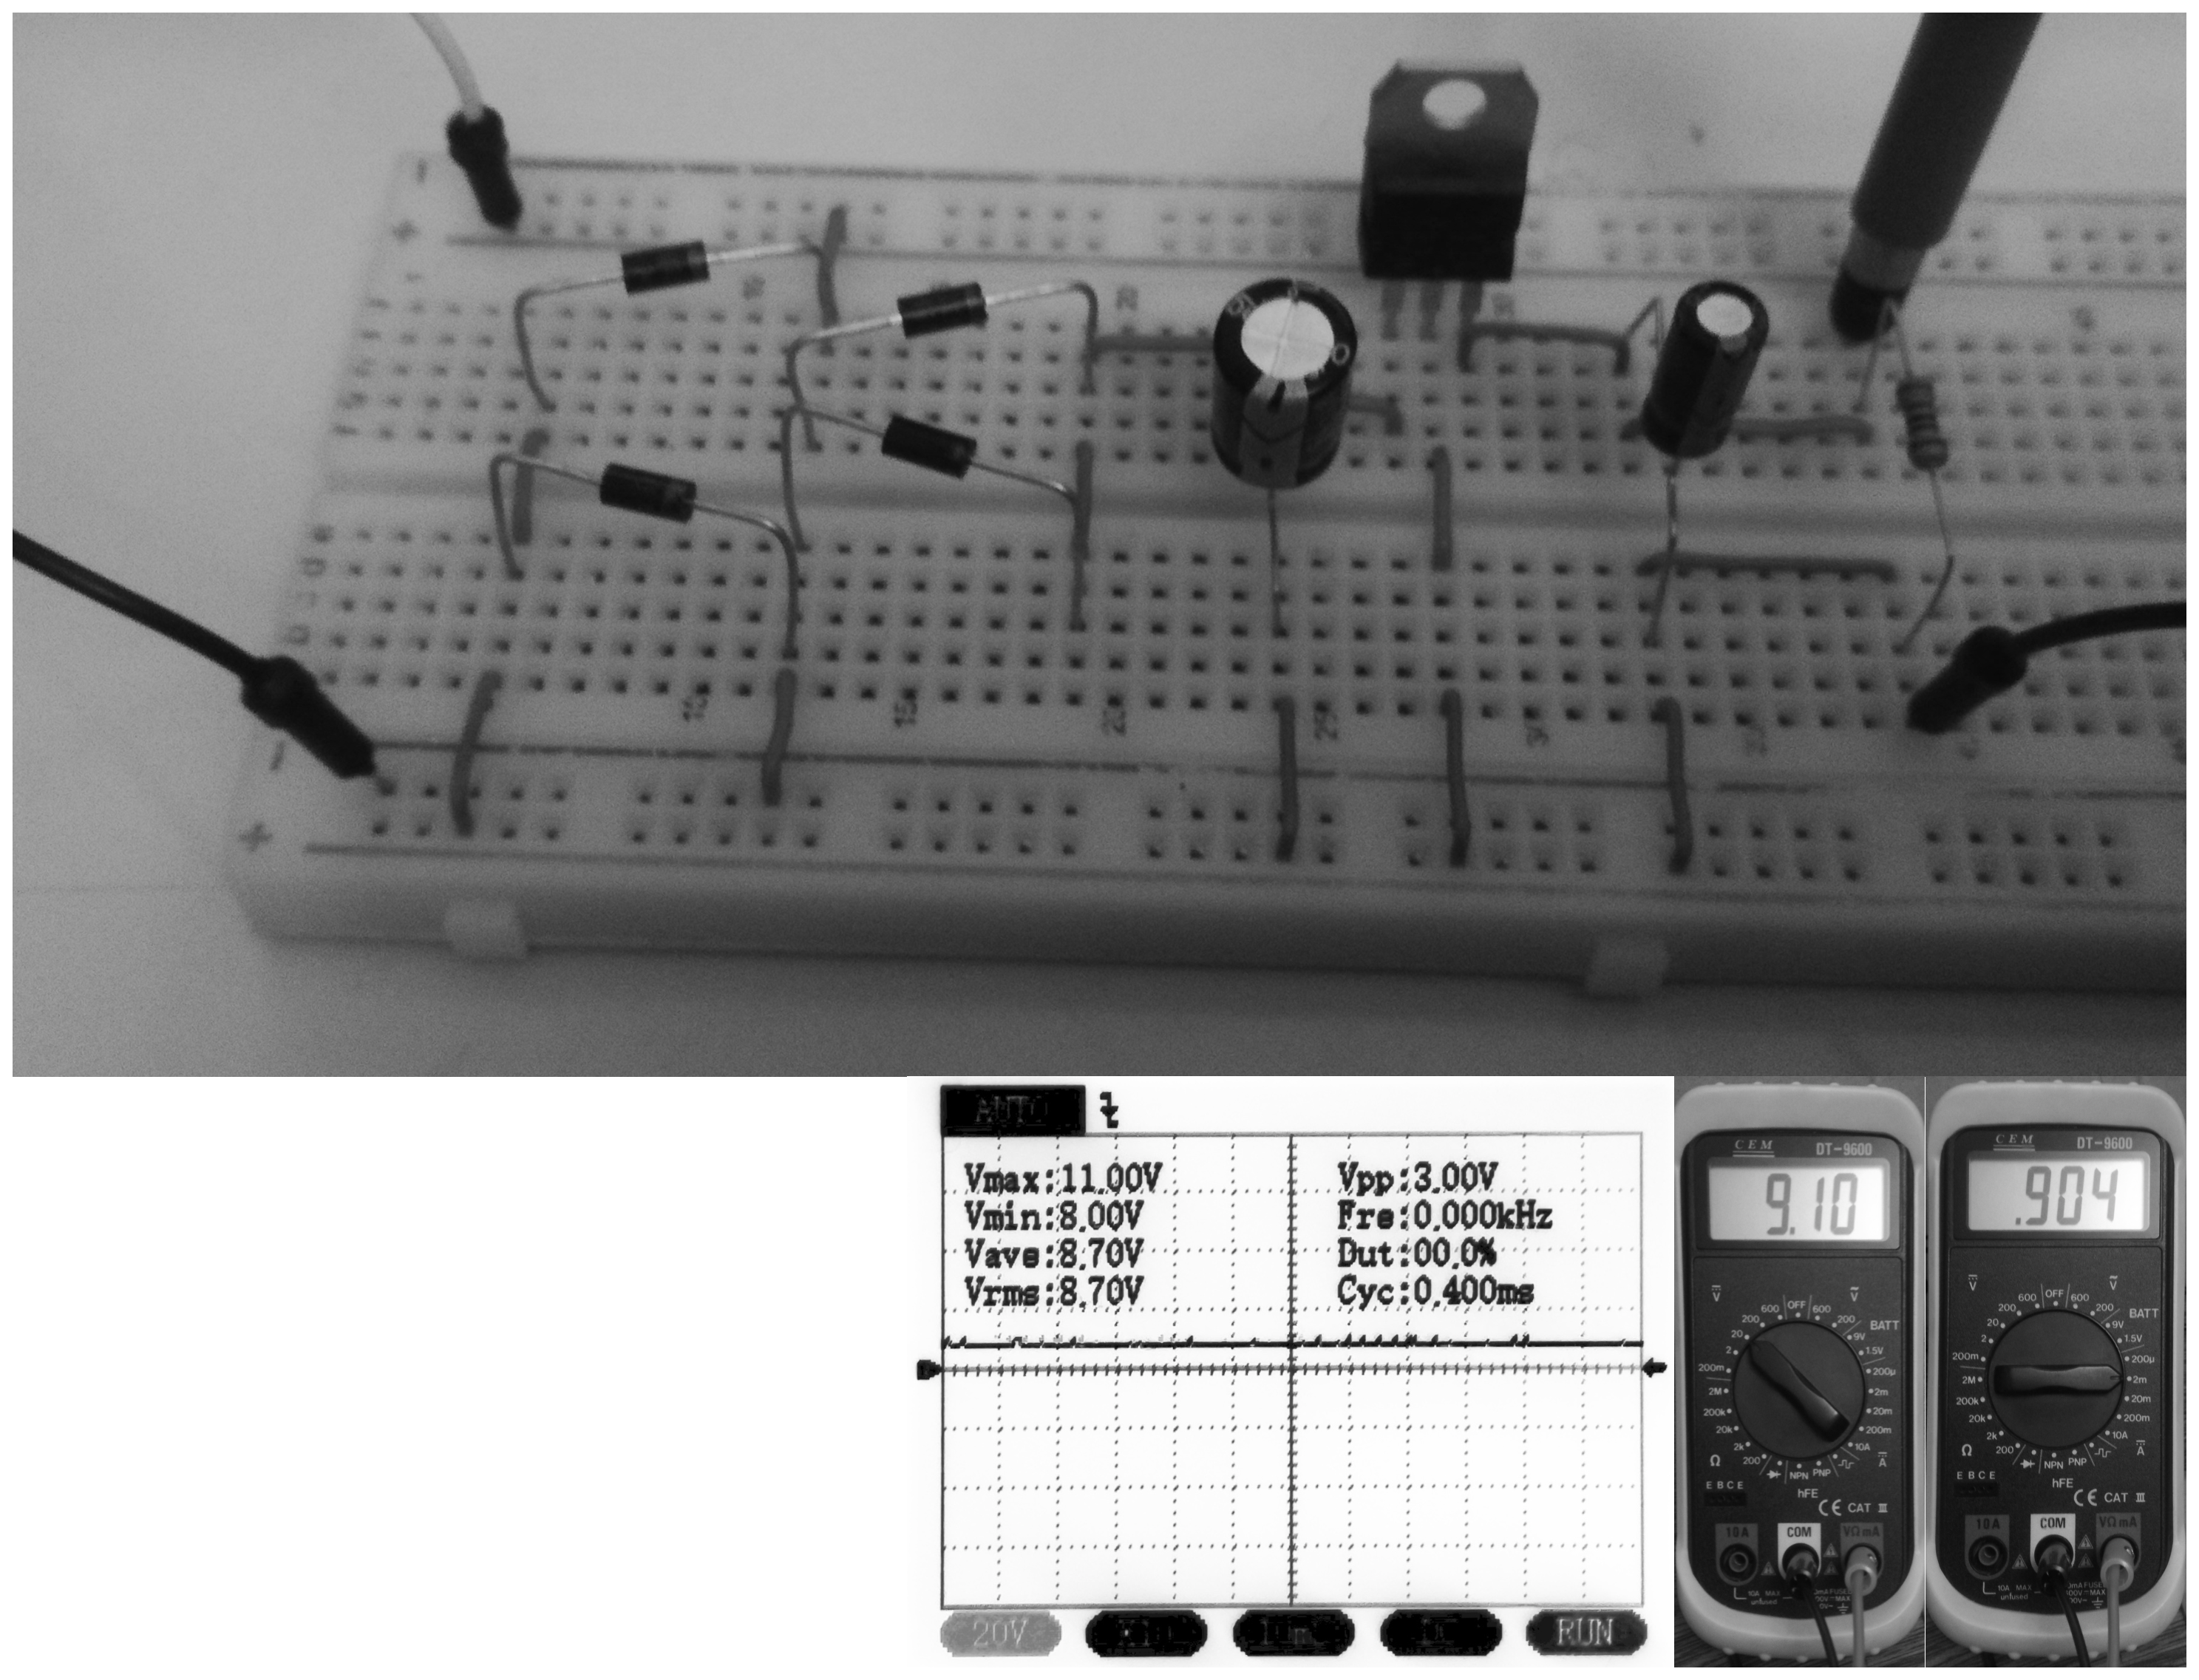
\includegraphics[scale=0.26]{fotos/09.regulador1.eps}
\caption{Regulador \textbf{L7809CV}, salida del osciloscopio\\
y medición de voltaje y corriente.}
\label{laboratorio11}
\end{figure}

\subsubsection{Laboratorio}
Se presenta el regulador \textbf{L7809CV} armado en laboratorio, su señal de
voltaje de salida en osciloscopio, así como su voltaje y corriente en un
multímetro para una resistencia de carga de $10[\text{k}\Omega]$ en la
\textbf{figura~\ref{laboratorio11}}.

